\documentclass[10pt,a4paper]{article}

\usepackage[T1]{fontenc}
\usepackage[utf8]{inputenc}
\usepackage{lmodern}
\usepackage{microtype}
\usepackage[a4paper,left=18mm,right=18mm,top=25mm,bottom=20mm,headheight=17mm,headsep=8mm,footskip=10mm]{geometry}
\usepackage{xcolor}
\usepackage{graphicx}
\usepackage{tabularx}
\usepackage{array}
\usepackage{booktabs}
\usepackage{enumitem}
\usepackage{titlesec}
\usepackage{tcolorbox}
\usepackage{fancyhdr}
\usepackage{lastpage}
\usepackage{tikz}
\usepackage{hyperref}
\hypersetup{hidelinks}
\usepackage[backend=biber,style=ieee,sorting=none]{biblatex}
\addbibresource{../ref.bib}

% -----------------------------------------------------------------------------
% Colours sampled/approximated from the original document
% -----------------------------------------------------------------------------
\definecolor{MetroBlue}{HTML}{23477F}
\definecolor{MetroOrange}{HTML}{F39200}
\definecolor{BodyText}{HTML}{202B3A}
\definecolor{Muted}{HTML}{65748A}
\definecolor{RuleGray}{HTML}{D3D6DA}
\definecolor{PanelGray}{HTML}{F1F2F4}
\definecolor{ReqPanel}{HTML}{E9EDF3}
\definecolor{ConfRed}{HTML}{C9252B}

\color{BodyText}
\setlength{\parindent}{0pt}
\setlength{\parskip}{0pt}
\renewcommand{\familydefault}{\sfdefault}

% -----------------------------------------------------------------------------
% Header and footer
% -----------------------------------------------------------------------------
\newcommand{\ConfidentialBox}{%
  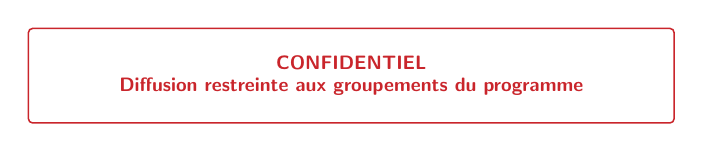
\begin{tikzpicture}[baseline=(current bounding box.center)]
    \node[draw=ConfRed, rounded corners=1.5pt, line width=.55pt,
      minimum width=82mm, minimum height=12mm, align=center,
      text=ConfRed, font=\bfseries\fontsize{6.7}{8}\selectfont, inner sep=2pt]
      {CONFIDENTIEL\\Diffusion restreinte aux groupements du programme};
  \end{tikzpicture}%
}
\pagestyle{fancy}
\fancyhf{}
\fancyhead[L]{\raisebox{1.5mm}{\color{Muted}\fontsize{7.2}{8.5}\selectfont
  Metropolis $\cdot$ Programme Renouvellement Signalisation $\cdot$ GSS}}
\fancyhead[R]{\ConfidentialBox}
\fancyfoot[R]{\color{Muted}\fontsize{7.5}{9}\selectfont\thepage\,/\,\pageref*{LastPage}}
\renewcommand{\headrulewidth}{0pt}
\renewcommand{\footrulewidth}{0pt}

% -----------------------------------------------------------------------------
% Section heading style
% -----------------------------------------------------------------------------
\titleformat{\section}
  {\normalfont\bfseries\Large\color{MetroBlue}}
  {\textcolor{MetroOrange}{\thesection.}}{0.55em}{}
\titlespacing*{\section}{0pt}{0pt}{8pt}

% -----------------------------------------------------------------------------
% Requirement panels: light blue-grey box with a blue bar on the left,
% bold "Requirement N:" label followed by the requirement in italics.
% Usage: \begin{requirement} ... \end{requirement}
%        \begin{requirement}[req:label] ... \end{requirement}  (for \ref)
% -----------------------------------------------------------------------------
\newcounter{requirement}
\newtcolorbox{requirementbox}{
  colback=ReqPanel,
  colframe=MetroBlue,
  sharp corners,
  boxrule=0pt, leftrule=2.5pt,
  left=3.5mm,right=4mm,top=2.2mm,bottom=2.2mm,
  before skip=7pt, after skip=6pt,
  fontupper=\small
}
\newenvironment{requirement}[1][]{%
  \refstepcounter{requirement}%
  \if\relax\detokenize{#1}\relax\else\label{#1}\fi
  \begin{requirementbox}%
  {\bfseries\color{MetroBlue}Requirement \therequirement:}\hspace{.6em}\itshape
}{%
  \end{requirementbox}%
}
% Requirement with a custom number, e.g. "Requirement EXIT 1:"
% Usage: \begin{namedrequirement}{EXIT 1} ... \end{namedrequirement}
%        \begin{namedrequirement}{EXIT 1}[req:exit1] ...   (for \ref)
\makeatletter
\NewDocumentEnvironment{namedrequirement}{m o}{%
  \def\@currentlabel{#1}%
  \IfValueT{#2}{\label{#2}}%
  \begin{requirementbox}%
  {\bfseries\color{MetroBlue}Requirement #1:}\hspace{.6em}\itshape
}{%
  \end{requirementbox}%
}
\makeatother

% Numbered conditions inside a requirement (1., 2., ...)
\newlist{conditions}{enumerate}{1}
\setlist[conditions]{label=\arabic*., leftmargin=6mm, labelsep=2mm,
  itemsep=1.5pt, topsep=3pt, parsep=0pt, partopsep=0pt}

\begin{document}

% =============================================================================
% PAGE 1 — COVER / DOCUMENT INFORMATION
% =============================================================================
\thispagestyle{fancy}

\vspace*{1mm}
\noindent
\begin{minipage}[c]{0.59\textwidth}
  
\includegraphics[height=1.4cm,keepaspectratio]{../logo/LogoMetropolis.pdf}
\end{minipage}%
\begin{minipage}[c]{0.40\textwidth}
  \raggedleft
  
\includegraphics[height=0.45cm,keepaspectratio]{../logo/LogoProver.pdf}
\end{minipage}

\vspace{12mm}
{\color{MetroOrange}\bfseries\fontsize{8.2}{10}\selectfont
  P R O G R A M M E\quad R E N O U V E L L E M E N T\quad S I G N A L I S A T I O N\par}

\vspace{4mm}
{\color{MetroBlue}\bfseries\fontsize{25}{30}\selectfont
  Generic Safety Specification for\\[-1mm]
  Metropolis GA package\par}

\vspace{2mm}
{\color{Muted}\fontsize{10.5}{13}\selectfont Version 2.1, 2026-11-04\par}

\vspace{10mm}
{\color{Muted}\bfseries\fontsize{7.5}{9}\selectfont REVISION HISTORY\par}
\vspace{2mm}
\renewcommand{\arraystretch}{1.55}
\begin{tabularx}{\textwidth}{@{}>{\raggedright\arraybackslash}p{0.13\textwidth}
  >{\raggedright\arraybackslash}p{0.17\textwidth}
  >{\raggedright\arraybackslash}p{0.13\textwidth}
  >{\raggedright\arraybackslash}X@{}}
  \textcolor{Muted}{\bfseries\fontsize{7}{8}\selectfont VERSION} &
  \textcolor{Muted}{\bfseries\fontsize{7}{8}\selectfont DATE} &
  \textcolor{Muted}{\bfseries\fontsize{7}{8}\selectfont AUTHOR} &
  \textcolor{Muted}{\bfseries\fontsize{7}{8}\selectfont CHANGE} \\
  \midrule
  0.1 & 2022-06-15 & DF & Draft version for review \\
  \midrule
  1.0 & 2022-08-19 & DF & First version \\
  \midrule
  1.1 & 2022-10-25 & HF & Adding buffer stop case to req. 6 \\
  \midrule
  2.0 & 2026-11-3 & G & Demanding line input and line vacancy for exit signal case in req. 6   \\
  \midrule
  2.1 & 2026-11-4 & G & Adding req. EXIT 1 and EXIT 2 \\
  \bottomrule
\end{tabularx}
\renewcommand{\arraystretch}{1}

\vspace{4mm}
\begin{tcolorbox}[
  colback=PanelGray,colframe=PanelGray,boxrule=0pt,arc=2mm,
  left=4mm,right=4mm,top=3mm,bottom=2.5mm]
  {\color{Muted}\bfseries\fontsize{7.5}{9}\selectfont CONTENTS\par}
  \vspace{2mm}
  \begin{enumerate}[label=\textcolor{MetroOrange}{\bfseries\arabic*.},
    leftmargin=5mm,labelsep=2mm,itemsep=2.5mm,topsep=0pt,parsep=0pt]
    \item Introduction
    \item Safety Requirements
  \end{enumerate}
\end{tcolorbox}

\newpage

% =============================================================================
% PAGE 2 — SAFETY REQUIREMENTS
% =============================================================================
\section{Introduction}
This is the informal Generic Safety Specification for the Metropolis GA package.

\vspace{9mm}
\section{Safety Requirements}

\begin{requirement}[req:proceed]
  If a signal is commanded to proceed, then one of the following holds:
  \begin{conditions}
    \item It is not an exit signal and there is a unique set route that starts at the signal.
    \item It is an exit signal, it is end locked and the track circuit behind it is clear of occupancy.
  \end{conditions}
\end{requirement}

The set route beginning at the signal is the one that is supposed to be safe for a train to travel, so we need to ensure that there is such a route in place when a signal shows proceed. Requirements 2-6 will ensure that this route actually is safe to travel,

\begin{requirement}[req:sharing]
  Route sections which share tracks cannot be locked at the same time.
\end{requirement}

\begin{requirement}[req:switches]
  If a signal that is the start of a set route is commanded to proceed, then the switches in the route are detected in their correct positions.
\end{requirement}

The switchess in the route are given by the relations Switch In Normal/Reverse relations from the route sections in the route.

\begin{requirement}[req:tracks]
  If a signal that is the start of a set route is commanded to proceed, then all tracks in the route are clear from occupancy.
\end{requirement}

The tracks in the route are given by the tracks in the route sections in the route.

\begin{requirement}[req:flank]
  If a signal that is the start of a set route is commanded to proceed, then, for every switch in the route, there is a protection area that is protective (flank protection).
\end{requirement}

Flank protection deals with two things. First, it stop other trains entering the set route from the flank. In order for that to be possible, there has to be switches in the route. It is then possible for a train to enter the set route from the leg of the switch that is not part of the route. In other words, there is a path ending at that switch. The protection area is assumed to give positions for other switches in that path such that those positions makes it impossible for other trains to enter the set route. That the area is protective means that those switches are detected in the protective positions. It is also assumed that the tracks given in the protection area includes all the tracks in the path. If no switch positions are given, then it is assumed that the path starts in a signal that is directed towards the set route. Second, flank protection also ensures that the tracks between the set route and the protective switch or signal (referred to as protection objects)are clear from occupancy. In other words, no train is hiding between the route and the protection objects.

\begin{requirement}[req:front]
  If a signal that is the start of a set route is commanded to proceed, then either the route ends at a buffer stop, ends at an exit signal with the line input set and a vacant line track, the end signal is commanded to proceed, or there is a protection area for the end signal that is protective (front protection).
\end{requirement}

Front protection is similar to flank protection but it stops trains from entering the set route in the front, from the end signal.

% The original starts page 3 at Requirement 7. Remove this \newpage once
% you add content above, if it leaves too much white space.
\newpage

% =============================================================================
% PAGE 3 — SAFETY REQUIREMENTS (continued)
% =============================================================================
\begin{requirement}[req:move]
  A switch cannot be moved if any of the following holds:
  \begin{conditions}
    \item The switch is located in a locked route section.
    \item The switch is a protective object to another switch that is located in a locked route section.
    \item The switch is a protective object to an end locked signal that is not commanded to proceed.
  \end{conditions}
\end{requirement}

This requirement ensures that switches will not change positions in the set route as the train traverses it.

\begin{requirement}[req:rtr-occupied]
  If a route section becomes ready to release, then it is occupied.
\end{requirement}

This is to ensure that a route section cannot release before it has been occupied.

\begin{requirement}[req:rtr-locked]
  If a route section is ready to release, then it is locked.
\end{requirement}

This together with requirement 8 ensures that only occupancy of locked route sections make them ready for release. It also ensures that Ready To Release is reset when the route section releases.

\begin{requirement}[req:release]
  If a route section releases, then it is clear of occupancy and ready to release.
\end{requirement}

The requirement ensures that the route section releases only after the train has passed it, provided it does not reverse direction.



\begin{namedrequirement}{EXIT 1}[req:exit1]
    If the line output of an exit signal is set, then all of the
    following holds:
    \begin{conditions}
        \item The signal is not end locked.
        \item The signal is not commanded to proceed.
        \end{conditions}
\end{namedrequirement}
The requirement ensures that if a station A tells it's neighbourg station B it isn't using the line, then indeed it hasn't reserved that line nor sent a train trought line
\begin{namedrequirement}{EXIT 2}[req:exit2]
    If an exit signal is commanded to proceed, then all of the
    following holds:
    \begin{conditions}
        \item The signal is end locked.
        \item The line inputs is set.
        \item The line track circuit is vacant.
        \end{conditions}
\end{namedrequirement}
The requirement ensures that if a station A is sending a train to another station B, then A has reserved the line, A has already received a message from B saying it is not using the line and the line between the stations is not being used


% -----------------------------------------------------------------------------
% New requirements go here — numbering continues automatically (11, 12, ...):
%
% \begin{requirement}[req:my-new-req]
%   If ..., then ...
% \end{requirement}
%
% Explanation of the requirement.
% -----------------------------------------------------------------------------

\end{document}